\chapter{Návrh}

\indent

Kdybychom navrhovali SOAP službu, vzali bychom všechny případy užití (use cases) a~k~nim zpřístupnili
konkrétní metody. V REST je návrh trochu složitejší.
Musíme nejprve identifikovat všechny zdroje, se kterými se bude pracovat a~umožnit
k~nim přístup pomocí standardizovaných metod. V návrhu vycházíme ze tří ustálených modelů:

\begin{itemize}
\item Doménový model
\item Datový model
\item Use case diagramy
\end{itemize}

První dva modely nám slouží k identifikování jednotlivých zdrojů.
Doménový model poskytuje klíčové entity a vztahy mezi nimi.
Jde o~vysoko-úrovňový pohled na problematiku. Nezbytné detaily dořešíme pomocí datového modelu. 
Akce, které nejdou pokrýt pomocí standartních metod manipulujících se zdroji, nám mohou poskytnout use case diagramy.
My si vystačíme s případy užití a jejich diagramem, který jsme zpracovali v sekci~\ref{sec:use_case}. 
Diagramy všech tří modelů jsou tedy v této práci zpracovány.

\subsection{Doménový model}

\indent

Tvorba doménového modelu (na obrázku~\ref{fig:domain_model}) vychází ze zadání. Obsahuje následující entity,
jenž modelují základní představu o systému.

\begin{description}
  \item[Uživatel (user)]
  Uživatel je identifikován emailem. Přihlašuje se heslem nebo api klíčem (více v kapitole X).
  Zároveň může nabývat jednou ze tří rolí (\texttt{club},\texttt{organizer} a \texttt{admin}).
  \item[Oddíl (club)]
  Oddíl je logický prvek, který zastřešuje více týmů. Správu oddílu provádí klubový účet.
  \item[Tým (team)]
  Tým je vázán na oddíl. Jeho identifikátory jsou divize a stupeň týmu (např. A-tým).
  \item[Divize (division)]
  Kategorie, ve které se pořádají turnaje, nebo je složen tým. % Například ženský tým je v divizi \texttt{women}.
  \item[Turnaj (tournament)]
    Turnaj nabývá několika stavů (stavový diagram na obrázku~\ref{fig:state_tournament}).
    Po vytvoření turnaje lze až do potvrzení (příznak \texttt{ready}) měnit týmy, které se turnaje zúčastní.
    Po něm mohou klubové účty odevzdávat soupisky za svoje týmy a na turnaji je možné aktivovat aktivovat zápasy. Ve chvíli,
    kdy všechny týmy odevzdají svoje hodnocení SOTG a je známo finální pořadí týmů,
    lze turnaj ukončit (příznak \texttt{terminated}). Do té doby skryté výsledky hodnocení SOTG se stanou veřejnými.
    Turnaj je spravován administrátorem nebo uživatelem s rolí \texttt{organizer} (tzv.~organizátor).
    \begin{figure}[ht!]
      \centering
      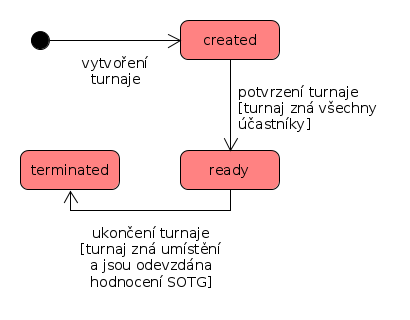
\includegraphics[width=90mm]{./images/stavovy-diagram-turnaj.png}
      \caption{Stavový diagram turnaje.\label{overflow}}
      \label{fig:state_tournament}
    \end{figure}
  \item[Zápas (match)]
    Zápas má stejně jako turnaj tři stavy (obrázek ~\ref{fig:state_match}). Aktivováním zápasu je umožněno zadat výsledek
    nebo postupně vkládat jednotlivé body. Ukončením (příznak \texttt{terminated}) se uloží výsledky a ty se následně promítnou
    v dalším postupu turnajem (vítězný tým posune do dalšího zápasu, týmům se přidá výhra ve skupině apod.).
    \begin{figure}[ht!]
      \centering
      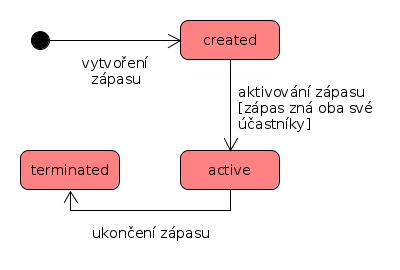
\includegraphics[width=90mm]{./images/stavovy-diagram-zapas.png}
      \caption{Stavový diagram zápasu.\label{overflow}}
      \label{fig:state_match}
    \end{figure}
  \item[Bod (point)]
    Zápas je složen z několika bodů. Každý bod je záznamem o skórování. Uchovává informaci, jaký hráč a komu nahrával.
    Zápas může být ukončen, i bez jednotlivých bodů, zadáním výsledného skóre.
  \item[Skupina (group)]
    Jde o několik týmů, které hrají zápasy pouze mezi sebou. Po odehrání všech utkání ve skupině se podle pravidel určí pořadí a podle něj se týmy posunou turnajem dál.
  \item[Hřiště (field)]
    Každé utkání se musí někde hrát. K tomu slouží hřiště.
  \item[Hodnocení SOTG (SOTG score)]
    Po každém utkání musí tým ohodnotit soupeře hodnocením Spirit of the Game. Jde o číselné vyjádření na stupnici od 0 do 10.
\end{description}

\begin{figure}[ht!]
\centering
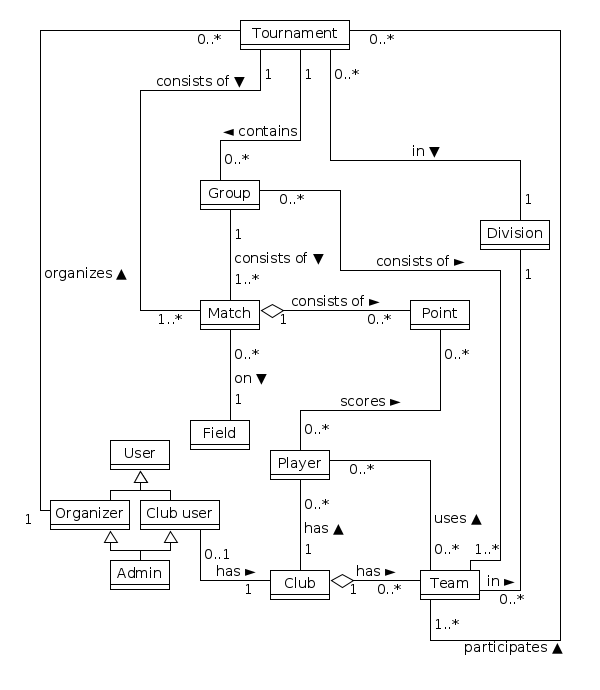
\includegraphics[width=130mm]{./images/domenovy-model.png}
\caption{Doménový model.\label{overflow}}
\label{fig:domain_model}
\end{figure}

\subsection{Datový model}

\indent

Pro ujasnění entit a vazeb mezi nimi byl vhodný doménový model. Jeho konkrétní implementací je model datový.
Ten je dekomponován, tj. zbavení se M:N vazeb, a oproti doménovému modelu obsahuje nové
(relační) objekty, včetně atributů. Kompletní datový model je dostupný v příloze~\ref{appendix:data_model}.